\documentclass[11pt]{amsart}
\usepackage[a4paper,margin=1in]{geometry}
\usepackage{amssymb}
\usepackage{booktabs}
\usepackage{tikz}
\usepackage[font=small,labelfont=bf]{caption}
\usepackage[hidelinks]{hyperref}

\colorlet{copper}{orange!75!black}
\colorlet{inkmuted}{black!60}

\newtheorem{theorem}{Theorem}
\newtheorem{lemma}[theorem]{Lemma}
\theoremstyle{remark}
\newtheorem{remark}[theorem]{Remark}

\title{Five From Inverse Pairs}
\author{Vamshi Jandhyala}
\address{London, United Kingdom}
\email{vamshi.jandhyala@gmail.com}

\begin{document}

\begin{abstract}
For a prime $p$ let $S(p)=\sum_{a=1}^{p-1}(a\bar a)^{-1/2}$, where $\bar a$ is the inverse of $a$ modulo $p$ in $\{1,\dots,p-1\}$. A question on Mathematics Stack Exchange asked whether $S(p)\to5$, as computations suggest. We prove $S(p)=5+O_\varepsilon(p^{-1/8+\varepsilon})$. The proof compares the inverse pairs $(a,\bar a)$ with all pairs $(a,b)$ under each hyperbola $ab=X$: Weil's bound for Kloosterman sums controls large $X$, the divisor bound controls small $X$, and the sum over all pairs is $(\sum_{a<p}a^{-1/2})^2/p\to4$. Everything except Weil's bound, which enters as a stated hypothesis, is formally verified in Lean~4.
\end{abstract}

\maketitle

\section{The question}

Pick a prime $p$ and pair each number $a$ from $1$ to $p-1$ with its inverse $\bar a$ modulo $p$, the number in the same range with $a\bar a\equiv1\pmod p$. For $p=7$ the pairs are $(1,1)$, $(2,4)$, $(3,5)$, $(4,2)$, $(5,3)$ and $(6,6)$. Add up $1/\sqrt{a\bar a}$:
\[
S(p)=\sum_{a=1}^{p-1}\frac1{\sqrt{a\,\bar a}},\qquad S(7)=1+\frac2{\sqrt8}+\frac2{\sqrt{15}}+\frac16\approx2.39 .
\]
In August 2026 Nilotpal Kanti Sinha asked on Mathematics Stack Exchange~\cite{MSE} whether $S(p)\to5$, having computed $S(p)$ for primes up to about $2\times10^6$ and sampled it further. Table~\ref{tab:Sp} shows the drift. Before reading on, try to guess where a $5$ could come from.

\begin{table}[ht]
\centering
\begin{tabular}{rlll}
\toprule
$p$ & $S(p)$ & $C(p)$ & $S(p)-1-C(p)$\\
\midrule
$1\,009$ & $4.470474$ & $3.816281$ & $-0.346$\\
$10\,007$ & $4.875732$ & $3.941621$ & $-0.066$\\
$100\,003$ & $4.955035$ & $3.981529$ & $-0.026$\\
$1\,000\,003$ & $4.980697$ & $3.994159$ & $-0.013$\\
$10\,000\,019$ & $4.988406$ & $3.998153$ & $-0.0097$\\
$100\,000\,007$ & $5.001501$ & $3.999416$ & $+0.0021$\\
\bottomrule
\end{tabular}
\caption{$S(p)$, the full-grid sum $C(p)$ of~\eqref{eq:C}, and the difference $S(p)-1-C(p)$, for primes near powers of ten.}
\label{tab:Sp}
\end{table}

Two comments on the question found the shape of an answer. Bruno Andrades noted that the term $a=1$ is exactly $1$ and that $\iint_{[0,1]^2}(xy)^{-1/2}\,dx\,dy=4$: if the points $(a/p,\bar a/p)$ spread evenly over the unit square, the other terms, each $\frac1pf(a/p,\bar a/p)$ with $f(x,y)=(xy)^{-1/2}$, would add up to about $4$. Jyrki Lahtonen pointed to Kloosterman sums, the standard tool for that even spread. A third comment, by the user zhoraster, reported that an AI model had proved $S(p)=5+O(p^{-1/6+\varepsilon})$, but no proof was posted with it (as of 10 October 2026). Here is a proof that can be checked.

\begin{theorem}\label{thm:five}
For every $\varepsilon>0$ there is $K_\varepsilon$ with $|S(p)-5|\le K_\varepsilon\,p^{-1/8+\varepsilon}$ for every prime $p$. In particular $S(p)\to5$.
\end{theorem}

The heuristic cannot be the whole proof. Equidistribution of $(a/p,\bar a/p)$ controls sums of bounded continuous functions, and $(xy)^{-1/2}$ blows up along both axes. The work is in showing that the small products $a\bar a$, where the function is large, contribute what they should.

\section{The plan: compare with all pairs}

Rather than comparing $S(p)$ with an integral, compare it with the same sum over \emph{all} pairs $(a,b)$, scaled by $1/p$, since one pair in $p$ is an inverse pair on average:
\begin{equation}\label{eq:C}
C(p)=\frac1p\sum_{a,b=1}^{p-1}\frac1{\sqrt{ab}}=\frac1p\Bigl(\sum_{a=1}^{p-1}\frac1{\sqrt a}\Bigr)^2 .
\end{equation}
The right-hand side factors because $\sqrt{ab}=\sqrt a\sqrt b$, and it is easy to evaluate.

\begin{lemma}\label{lem:grid}
$|C(p)-4|\le8/\sqrt p$.
\end{lemma}

\begin{proof}
For $a\ge1$, $2(\sqrt{a+1}-\sqrt a)\le1/\sqrt a\le2(\sqrt a-\sqrt{a-1})$, because $\sqrt{a\pm1}-\sqrt a=\pm1/(\sqrt{a\pm1}+\sqrt a)$. Summing over $1\le a\le p-1$, both sides telescope: $2\sqrt p-2\le\sum_{a<p}a^{-1/2}\le2\sqrt{p-1}$. Squaring and dividing by $p$ gives $4-8/\sqrt p\le C(p)\le4$.
\end{proof}

So $C(p)\to4$, and Theorem~\ref{thm:five} says that $S(p)-1$ and $C(p)$ have the same limit. The table shows $S(p)-1-C(p)$ shrinking faster than $S(p)-5$, since $C(p)$ already carries the slow correction $4\zeta(\tfrac12)/\sqrt p$.

Both sums depend only on products. For an integer $X$ let
\[
R(X)=\#\{2\le a\le p-1:\ a\bar a\le X\},\qquad T(X)=\#\{(a,b)\in[1,p-1]^2:\ ab\le X\},
\]
the inverse pairs (other than $(1,1)$) and all pairs under the hyperbola $xy=X$. Figure~\ref{fig:pairs} shows them for $p=101$ and $X=2000$: there are $50$ copper inverse pairs under the curve, and $T(2000)/101\approx50.9$. The heart of the proof is that $R(X)$ stays close to $T(X)/p$. Since $a\bar a\equiv1\pmod p$, every product other than $1$ is at least $p+1$, so $R(X)=0$ for $X\le p$; for larger $X$ there are two regimes.

\begin{figure}[ht]
\centering
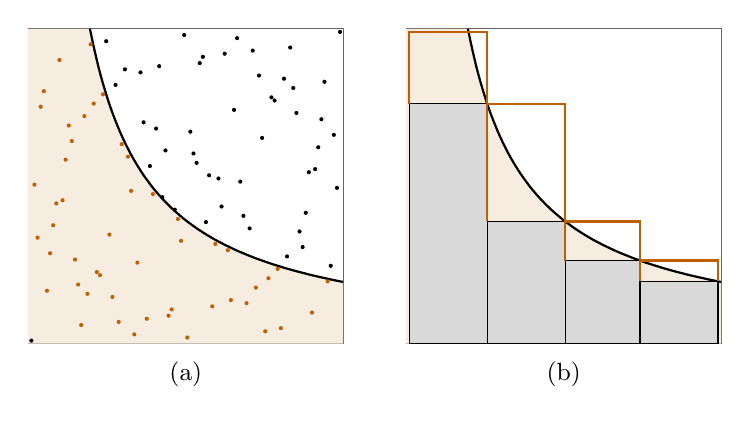
\begin{tikzpicture}
  \begin{scope}[shift={(0,0)}]
\draw[inkmuted] (0,0) rectangle (4.000,4.000);
\fill[copper!12] (0,0) -- (0,4.000) -- (0.784,4.000) -- (0.811,3.868) -- (0.838,3.744) -- (0.865,3.628) -- (0.891,3.519) -- (0.918,3.416) -- (0.945,3.319) -- (0.972,3.228) -- (0.999,3.141) -- (1.025,3.059) -- (1.052,2.981) -- (1.079,2.907) -- (1.106,2.837) -- (1.133,2.770) -- (1.159,2.706) -- (1.186,2.645) -- (1.213,2.586) -- (1.240,2.530) -- (1.267,2.477) -- (1.293,2.425) -- (1.320,2.376) -- (1.347,2.329) -- (1.374,2.283) -- (1.401,2.240) -- (1.427,2.198) -- (1.454,2.157) -- (1.481,2.118) -- (1.508,2.081) -- (1.535,2.044) -- (1.561,2.009) -- (1.588,1.975) -- (1.615,1.942) -- (1.642,1.911) -- (1.669,1.880) -- (1.695,1.850) -- (1.722,1.822) -- (1.749,1.794) -- (1.776,1.767) -- (1.803,1.740) -- (1.829,1.715) -- (1.856,1.690) -- (1.883,1.666) -- (1.910,1.643) -- (1.937,1.620) -- (1.963,1.598) -- (1.990,1.576) -- (2.017,1.555) -- (2.044,1.535) -- (2.071,1.515) -- (2.097,1.496) -- (2.124,1.477) -- (2.151,1.458) -- (2.178,1.440) -- (2.205,1.423) -- (2.231,1.406) -- (2.258,1.389) -- (2.285,1.373) -- (2.312,1.357) -- (2.339,1.341) -- (2.365,1.326) -- (2.392,1.311) -- (2.419,1.297) -- (2.446,1.283) -- (2.473,1.269) -- (2.499,1.255) -- (2.526,1.242) -- (2.553,1.229) -- (2.580,1.216) -- (2.607,1.204) -- (2.633,1.191) -- (2.660,1.179) -- (2.687,1.167) -- (2.714,1.156) -- (2.740,1.145) -- (2.767,1.134) -- (2.794,1.123) -- (2.821,1.112) -- (2.848,1.102) -- (2.874,1.091) -- (2.901,1.081) -- (2.928,1.071) -- (2.955,1.062) -- (2.982,1.052) -- (3.008,1.043) -- (3.035,1.033) -- (3.062,1.024) -- (3.089,1.016) -- (3.116,1.007) -- (3.142,0.998) -- (3.169,0.990) -- (3.196,0.982) -- (3.223,0.973) -- (3.250,0.965) -- (3.276,0.957) -- (3.303,0.950) -- (3.330,0.942) -- (3.357,0.934) -- (3.384,0.927) -- (3.410,0.920) -- (3.437,0.913) -- (3.464,0.906) -- (3.491,0.899) -- (3.518,0.892) -- (3.544,0.885) -- (3.571,0.878) -- (3.598,0.872) -- (3.625,0.865) -- (3.652,0.859) -- (3.678,0.853) -- (3.705,0.847) -- (3.732,0.841) -- (3.759,0.835) -- (3.786,0.829) -- (3.812,0.823) -- (3.839,0.817) -- (3.866,0.811) -- (3.893,0.806) -- (3.920,0.800) -- (3.946,0.795) -- (3.973,0.790) -- (4.000,0.784) -- (4.000,0) -- cycle;
\draw[thick] (0.784,4.000) -- (0.811,3.868) -- (0.838,3.744) -- (0.865,3.628) -- (0.891,3.519) -- (0.918,3.416) -- (0.945,3.319) -- (0.972,3.228) -- (0.999,3.141) -- (1.025,3.059) -- (1.052,2.981) -- (1.079,2.907) -- (1.106,2.837) -- (1.133,2.770) -- (1.159,2.706) -- (1.186,2.645) -- (1.213,2.586) -- (1.240,2.530) -- (1.267,2.477) -- (1.293,2.425) -- (1.320,2.376) -- (1.347,2.329) -- (1.374,2.283) -- (1.401,2.240) -- (1.427,2.198) -- (1.454,2.157) -- (1.481,2.118) -- (1.508,2.081) -- (1.535,2.044) -- (1.561,2.009) -- (1.588,1.975) -- (1.615,1.942) -- (1.642,1.911) -- (1.669,1.880) -- (1.695,1.850) -- (1.722,1.822) -- (1.749,1.794) -- (1.776,1.767) -- (1.803,1.740) -- (1.829,1.715) -- (1.856,1.690) -- (1.883,1.666) -- (1.910,1.643) -- (1.937,1.620) -- (1.963,1.598) -- (1.990,1.576) -- (2.017,1.555) -- (2.044,1.535) -- (2.071,1.515) -- (2.097,1.496) -- (2.124,1.477) -- (2.151,1.458) -- (2.178,1.440) -- (2.205,1.423) -- (2.231,1.406) -- (2.258,1.389) -- (2.285,1.373) -- (2.312,1.357) -- (2.339,1.341) -- (2.365,1.326) -- (2.392,1.311) -- (2.419,1.297) -- (2.446,1.283) -- (2.473,1.269) -- (2.499,1.255) -- (2.526,1.242) -- (2.553,1.229) -- (2.580,1.216) -- (2.607,1.204) -- (2.633,1.191) -- (2.660,1.179) -- (2.687,1.167) -- (2.714,1.156) -- (2.740,1.145) -- (2.767,1.134) -- (2.794,1.123) -- (2.821,1.112) -- (2.848,1.102) -- (2.874,1.091) -- (2.901,1.081) -- (2.928,1.071) -- (2.955,1.062) -- (2.982,1.052) -- (3.008,1.043) -- (3.035,1.033) -- (3.062,1.024) -- (3.089,1.016) -- (3.116,1.007) -- (3.142,0.998) -- (3.169,0.990) -- (3.196,0.982) -- (3.223,0.973) -- (3.250,0.965) -- (3.276,0.957) -- (3.303,0.950) -- (3.330,0.942) -- (3.357,0.934) -- (3.384,0.927) -- (3.410,0.920) -- (3.437,0.913) -- (3.464,0.906) -- (3.491,0.899) -- (3.518,0.892) -- (3.544,0.885) -- (3.571,0.878) -- (3.598,0.872) -- (3.625,0.865) -- (3.652,0.859) -- (3.678,0.853) -- (3.705,0.847) -- (3.732,0.841) -- (3.759,0.835) -- (3.786,0.829) -- (3.812,0.823) -- (3.839,0.817) -- (3.866,0.811) -- (3.893,0.806) -- (3.920,0.800) -- (3.946,0.795) -- (3.973,0.790) -- (4.000,0.784);
\fill[black] (0.040,0.040) circle (0.75pt);
\fill[copper] (0.079,2.020) circle (0.75pt);
\fill[copper] (0.119,1.347) circle (0.75pt);
\fill[copper] (0.158,3.010) circle (0.75pt);
\fill[copper] (0.198,3.208) circle (0.75pt);
\fill[copper] (0.238,0.673) circle (0.75pt);
\fill[copper] (0.277,1.149) circle (0.75pt);
\fill[copper] (0.317,1.505) circle (0.75pt);
\fill[copper] (0.356,1.782) circle (0.75pt);
\fill[copper] (0.396,3.604) circle (0.75pt);
\fill[copper] (0.436,1.822) circle (0.75pt);
\fill[copper] (0.475,2.337) circle (0.75pt);
\fill[copper] (0.515,2.772) circle (0.75pt);
\fill[copper] (0.554,2.574) circle (0.75pt);
\fill[copper] (0.594,1.069) circle (0.75pt);
\fill[copper] (0.634,0.752) circle (0.75pt);
\fill[copper] (0.673,0.238) circle (0.75pt);
\fill[copper] (0.713,2.891) circle (0.75pt);
\fill[copper] (0.752,0.634) circle (0.75pt);
\fill[copper] (0.792,3.802) circle (0.75pt);
\fill[copper] (0.832,3.050) circle (0.75pt);
\fill[copper] (0.871,0.911) circle (0.75pt);
\fill[copper] (0.911,0.871) circle (0.75pt);
\fill[copper] (0.950,3.168) circle (0.75pt);
\fill[black] (0.990,3.842) circle (0.75pt);
\fill[copper] (1.030,1.386) circle (0.75pt);
\fill[copper] (1.069,0.594) circle (0.75pt);
\fill[black] (1.109,3.287) circle (0.75pt);
\fill[copper] (1.149,0.277) circle (0.75pt);
\fill[copper] (1.188,2.535) circle (0.75pt);
\fill[black] (1.228,3.485) circle (0.75pt);
\fill[copper] (1.267,2.376) circle (0.75pt);
\fill[copper] (1.307,1.941) circle (0.75pt);
\fill[copper] (1.347,0.119) circle (0.75pt);
\fill[copper] (1.386,1.030) circle (0.75pt);
\fill[black] (1.426,3.446) circle (0.75pt);
\fill[black] (1.465,2.812) circle (0.75pt);
\fill[copper] (1.505,0.317) circle (0.75pt);
\fill[black] (1.545,2.257) circle (0.75pt);
\fill[copper] (1.584,1.901) circle (0.75pt);
\fill[black] (1.624,2.733) circle (0.75pt);
\fill[black] (1.663,3.525) circle (0.75pt);
\fill[black] (1.703,1.861) circle (0.75pt);
\fill[black] (1.743,2.455) circle (0.75pt);
\fill[copper] (1.782,0.356) circle (0.75pt);
\fill[copper] (1.822,0.436) circle (0.75pt);
\fill[black] (1.861,1.703) circle (0.75pt);
\fill[copper] (1.901,1.584) circle (0.75pt);
\fill[copper] (1.941,1.307) circle (0.75pt);
\fill[black] (1.980,3.921) circle (0.75pt);
\fill[copper] (2.020,0.079) circle (0.75pt);
\fill[black] (2.059,2.693) circle (0.75pt);
\fill[black] (2.099,2.416) circle (0.75pt);
\fill[black] (2.139,2.297) circle (0.75pt);
\fill[black] (2.178,3.564) circle (0.75pt);
\fill[black] (2.218,3.644) circle (0.75pt);
\fill[black] (2.257,1.545) circle (0.75pt);
\fill[black] (2.297,2.139) circle (0.75pt);
\fill[copper] (2.337,0.475) circle (0.75pt);
\fill[copper] (2.376,1.267) circle (0.75pt);
\fill[black] (2.416,2.099) circle (0.75pt);
\fill[black] (2.455,1.743) circle (0.75pt);
\fill[black] (2.495,3.683) circle (0.75pt);
\fill[copper] (2.535,1.188) circle (0.75pt);
\fill[copper] (2.574,0.554) circle (0.75pt);
\fill[black] (2.614,2.970) circle (0.75pt);
\fill[black] (2.653,3.881) circle (0.75pt);
\fill[black] (2.693,2.059) circle (0.75pt);
\fill[black] (2.733,1.624) circle (0.75pt);
\fill[copper] (2.772,0.515) circle (0.75pt);
\fill[black] (2.812,1.465) circle (0.75pt);
\fill[black] (2.851,3.723) circle (0.75pt);
\fill[copper] (2.891,0.713) circle (0.75pt);
\fill[black] (2.931,3.406) circle (0.75pt);
\fill[black] (2.970,2.614) circle (0.75pt);
\fill[copper] (3.010,0.158) circle (0.75pt);
\fill[copper] (3.050,0.832) circle (0.75pt);
\fill[black] (3.089,3.129) circle (0.75pt);
\fill[black] (3.129,3.089) circle (0.75pt);
\fill[copper] (3.168,0.950) circle (0.75pt);
\fill[copper] (3.208,0.198) circle (0.75pt);
\fill[black] (3.248,3.366) circle (0.75pt);
\fill[black] (3.287,1.109) circle (0.75pt);
\fill[black] (3.327,3.762) circle (0.75pt);
\fill[black] (3.366,3.248) circle (0.75pt);
\fill[black] (3.406,2.931) circle (0.75pt);
\fill[black] (3.446,1.426) circle (0.75pt);
\fill[black] (3.485,1.228) circle (0.75pt);
\fill[black] (3.525,1.663) circle (0.75pt);
\fill[black] (3.564,2.178) circle (0.75pt);
\fill[copper] (3.604,0.396) circle (0.75pt);
\fill[black] (3.644,2.218) circle (0.75pt);
\fill[black] (3.683,2.495) circle (0.75pt);
\fill[black] (3.723,2.851) circle (0.75pt);
\fill[black] (3.762,3.327) circle (0.75pt);
\fill[copper] (3.802,0.792) circle (0.75pt);
\fill[black] (3.842,0.990) circle (0.75pt);
\fill[black] (3.881,2.653) circle (0.75pt);
\fill[black] (3.921,1.980) circle (0.75pt);
\fill[black] (3.960,3.960) circle (0.75pt);
\node[below, font=\small] at (2,-0.1) {(a)};
\end{scope}
\begin{scope}[shift={(4.8,0)}]
\draw[inkmuted] (0,0) rectangle (4.000,4.000);
\fill[copper!12] (0,0) -- (0,4.000) -- (0.784,4.000) -- (0.811,3.868) -- (0.838,3.744) -- (0.865,3.628) -- (0.891,3.519) -- (0.918,3.416) -- (0.945,3.319) -- (0.972,3.228) -- (0.999,3.141) -- (1.025,3.059) -- (1.052,2.981) -- (1.079,2.907) -- (1.106,2.837) -- (1.133,2.770) -- (1.159,2.706) -- (1.186,2.645) -- (1.213,2.586) -- (1.240,2.530) -- (1.267,2.477) -- (1.293,2.425) -- (1.320,2.376) -- (1.347,2.329) -- (1.374,2.283) -- (1.401,2.240) -- (1.427,2.198) -- (1.454,2.157) -- (1.481,2.118) -- (1.508,2.081) -- (1.535,2.044) -- (1.561,2.009) -- (1.588,1.975) -- (1.615,1.942) -- (1.642,1.911) -- (1.669,1.880) -- (1.695,1.850) -- (1.722,1.822) -- (1.749,1.794) -- (1.776,1.767) -- (1.803,1.740) -- (1.829,1.715) -- (1.856,1.690) -- (1.883,1.666) -- (1.910,1.643) -- (1.937,1.620) -- (1.963,1.598) -- (1.990,1.576) -- (2.017,1.555) -- (2.044,1.535) -- (2.071,1.515) -- (2.097,1.496) -- (2.124,1.477) -- (2.151,1.458) -- (2.178,1.440) -- (2.205,1.423) -- (2.231,1.406) -- (2.258,1.389) -- (2.285,1.373) -- (2.312,1.357) -- (2.339,1.341) -- (2.365,1.326) -- (2.392,1.311) -- (2.419,1.297) -- (2.446,1.283) -- (2.473,1.269) -- (2.499,1.255) -- (2.526,1.242) -- (2.553,1.229) -- (2.580,1.216) -- (2.607,1.204) -- (2.633,1.191) -- (2.660,1.179) -- (2.687,1.167) -- (2.714,1.156) -- (2.740,1.145) -- (2.767,1.134) -- (2.794,1.123) -- (2.821,1.112) -- (2.848,1.102) -- (2.874,1.091) -- (2.901,1.081) -- (2.928,1.071) -- (2.955,1.062) -- (2.982,1.052) -- (3.008,1.043) -- (3.035,1.033) -- (3.062,1.024) -- (3.089,1.016) -- (3.116,1.007) -- (3.142,0.998) -- (3.169,0.990) -- (3.196,0.982) -- (3.223,0.973) -- (3.250,0.965) -- (3.276,0.957) -- (3.303,0.950) -- (3.330,0.942) -- (3.357,0.934) -- (3.384,0.927) -- (3.410,0.920) -- (3.437,0.913) -- (3.464,0.906) -- (3.491,0.899) -- (3.518,0.892) -- (3.544,0.885) -- (3.571,0.878) -- (3.598,0.872) -- (3.625,0.865) -- (3.652,0.859) -- (3.678,0.853) -- (3.705,0.847) -- (3.732,0.841) -- (3.759,0.835) -- (3.786,0.829) -- (3.812,0.823) -- (3.839,0.817) -- (3.866,0.811) -- (3.893,0.806) -- (3.920,0.800) -- (3.946,0.795) -- (3.973,0.790) -- (4.000,0.784) -- (4.000,0) -- cycle;
\draw[thick] (0.784,4.000) -- (0.811,3.868) -- (0.838,3.744) -- (0.865,3.628) -- (0.891,3.519) -- (0.918,3.416) -- (0.945,3.319) -- (0.972,3.228) -- (0.999,3.141) -- (1.025,3.059) -- (1.052,2.981) -- (1.079,2.907) -- (1.106,2.837) -- (1.133,2.770) -- (1.159,2.706) -- (1.186,2.645) -- (1.213,2.586) -- (1.240,2.530) -- (1.267,2.477) -- (1.293,2.425) -- (1.320,2.376) -- (1.347,2.329) -- (1.374,2.283) -- (1.401,2.240) -- (1.427,2.198) -- (1.454,2.157) -- (1.481,2.118) -- (1.508,2.081) -- (1.535,2.044) -- (1.561,2.009) -- (1.588,1.975) -- (1.615,1.942) -- (1.642,1.911) -- (1.669,1.880) -- (1.695,1.850) -- (1.722,1.822) -- (1.749,1.794) -- (1.776,1.767) -- (1.803,1.740) -- (1.829,1.715) -- (1.856,1.690) -- (1.883,1.666) -- (1.910,1.643) -- (1.937,1.620) -- (1.963,1.598) -- (1.990,1.576) -- (2.017,1.555) -- (2.044,1.535) -- (2.071,1.515) -- (2.097,1.496) -- (2.124,1.477) -- (2.151,1.458) -- (2.178,1.440) -- (2.205,1.423) -- (2.231,1.406) -- (2.258,1.389) -- (2.285,1.373) -- (2.312,1.357) -- (2.339,1.341) -- (2.365,1.326) -- (2.392,1.311) -- (2.419,1.297) -- (2.446,1.283) -- (2.473,1.269) -- (2.499,1.255) -- (2.526,1.242) -- (2.553,1.229) -- (2.580,1.216) -- (2.607,1.204) -- (2.633,1.191) -- (2.660,1.179) -- (2.687,1.167) -- (2.714,1.156) -- (2.740,1.145) -- (2.767,1.134) -- (2.794,1.123) -- (2.821,1.112) -- (2.848,1.102) -- (2.874,1.091) -- (2.901,1.081) -- (2.928,1.071) -- (2.955,1.062) -- (2.982,1.052) -- (3.008,1.043) -- (3.035,1.033) -- (3.062,1.024) -- (3.089,1.016) -- (3.116,1.007) -- (3.142,0.998) -- (3.169,0.990) -- (3.196,0.982) -- (3.223,0.973) -- (3.250,0.965) -- (3.276,0.957) -- (3.303,0.950) -- (3.330,0.942) -- (3.357,0.934) -- (3.384,0.927) -- (3.410,0.920) -- (3.437,0.913) -- (3.464,0.906) -- (3.491,0.899) -- (3.518,0.892) -- (3.544,0.885) -- (3.571,0.878) -- (3.598,0.872) -- (3.625,0.865) -- (3.652,0.859) -- (3.678,0.853) -- (3.705,0.847) -- (3.732,0.841) -- (3.759,0.835) -- (3.786,0.829) -- (3.812,0.823) -- (3.839,0.817) -- (3.866,0.811) -- (3.893,0.806) -- (3.920,0.800) -- (3.946,0.795) -- (3.973,0.790) -- (4.000,0.784);
\draw[fill=inkmuted!25] (0.040,0) rectangle (1.030,3.046);
\draw[copper, thick] (0.040,3.046) -- (0.040,3.960) -- (1.030,3.960) -- (1.030,3.046);
\draw[fill=inkmuted!25] (1.030,0) rectangle (2.020,1.553);
\draw[copper, thick] (1.030,1.553) -- (1.030,3.046) -- (2.020,3.046) -- (2.020,1.553);
\draw[fill=inkmuted!25] (2.020,0) rectangle (2.970,1.056);
\draw[copper, thick] (2.020,1.056) -- (2.020,1.553) -- (2.970,1.553) -- (2.970,1.056);
\draw[fill=inkmuted!25] (2.970,0) rectangle (3.960,0.792);
\draw[copper, thick] (2.970,0.792) -- (2.970,1.056) -- (3.960,1.056) -- (3.960,0.792);
\node[below, font=\small] at (2,-0.1) {(b)};
\end{scope}

\end{tikzpicture}
\caption{(a) The points $(a,\bar a)$ for $p=101$ and the hyperbola $xy=2000$. The $50$ copper points, those with $a\ge2$ under the curve, are counted by $R(2000)$. (b) Lemma~\ref{lem:stair} squeezes the region under the curve between two staircases of rectangles, here four columns wide: grey rectangles inside, copper outlines containing it. Lemma~\ref{lem:box} counts the inverse pairs in each rectangle.}
\label{fig:pairs}
\end{figure}

\section{Inverse pairs in rectangles}

Write $e_p(t)=e^{2\pi it/p}$ and, for residues $u,v$, let $K(u,v)=\sum_{x\ne0}e_p(ux+v\bar x)$ be the Kloosterman sum. Weil proved in 1948~\cite{Weil} that $|K(u,v)|\le2\sqrt p$ when $u,v\ne0$. This is the one result we quote and do not prove. We also need $K(0,0)=p-1$ and $K(0,v)=K(u,0)=-1$ for $u,v\ne0$, since $x\mapsto\bar x$ permutes the nonzero residues and $\sum_{y\ne0}e_p(vy)=-1$.

\begin{lemma}\label{lem:box}
Let $I,J\subseteq\{1,\dots,p-1\}$ be intervals and $N(I,J)$ the number of $a\in I$ with $\bar a\in J$. Then
\[
\Bigl|N(I,J)-\frac{|I|\,|J|}p\Bigr|\le3\sqrt p\,(1+\ln p)^2 .
\]
\end{lemma}

This is a standard estimate, a special case of Theorem~13 in Shparlinski's survey~\cite{Shp}; we include the short proof because the constant matters below.

\begin{proof}
Detecting $x\in I$ and $\bar x\in J$ with the orthogonality relation $\frac1p\sum_ue_p(ut)=[p\mid t]$ gives
\[
N(I,J)=\frac1{p^2}\sum_{u,v}\hat I(u)\,\hat J(v)\,K(u,v),\qquad \hat I(u)=\sum_{a\in I}e_p(-ua).
\]
Now write $K(u,v)=K'(u,v)-1+p\,[u=v=0]$, where $K'=K+1$ when $u,v\ne0$ and $K'=0$ otherwise; the three values of $K$ on the axes make this exact. The term $-1$ contributes $-\sum_u\hat I(u)\sum_v\hat J(v)=0$, because $\sum_u\hat I(u)=p\,[0\in I]=0$. The term $p[u=v=0]$ contributes $p|I||J|$. So
\[
N(I,J)-\frac{|I||J|}p=\frac1{p^2}\sum_{u,v\ne0}\hat I(u)\,\hat J(v)\,\bigl(K(u,v)+1\bigr),
\]
and $|K+1|\le2\sqrt p+1\le3\sqrt p$. For $u\ne0$, $\hat I(u)$ is a geometric series with ratio $z=e_p(-u)$, so $|\hat I(u)|\le2/|z-1|=1/|\sin(\pi u/p)|$. Jordan's inequality $\sin x\ge2x/\pi$ on $[0,\pi/2]$, applied to $\pi u/p$ or $\pi(p-u)/p$, gives $1/|\sin(\pi u/p)|\le\frac p2\bigl(\frac1u+\frac1{p-u}\bigr)$, so
\[
\sum_{u\ne0}|\hat I(u)|\le\frac p2\cdot2H_{p-1}\le p(1+\ln p),
\]
and the same for $\hat J$. Multiplying the bounds and dividing by $p^2$ finishes the proof.
\end{proof}

\section{Under the hyperbola}

\begin{lemma}\label{lem:stair}
Let $h,L\ge1$ with $Lh\ge p-1$. For every $X$,
\[
\Bigl|R(X)+1-\frac{T(X)}p\Bigr|\le3L\sqrt p\,(1+\ln p)^2+h .
\]
\end{lemma}

\begin{proof}
Cut $\{1,\dots,p-1\}$ into $L$ consecutive columns $I_\ell=[c_\ell,c_{\ell+1})$ of width at most $h$. On column $\ell$ put $m^+_\ell=\min(p-1,\lfloor X/c_\ell\rfloor)$ and $m^-_\ell=\min(p-1,\lfloor X/(c_{\ell+1}-1)\rfloor)$. For $a\in I_\ell$, the condition $\bar a\le m^-_\ell$ implies $a\bar a\le X$, which implies $\bar a\le m^+_\ell$. So the inverse pairs under the hyperbola in this column number between $N(I_\ell,[1,m^-_\ell])$ and $N(I_\ell,[1,m^+_\ell])$. Counting $a=1$ too, the left side of the lemma involves $R(X)+1$. The squeeze never used $b=\bar a$, so the pairs $(a,b)$ with $a\in I_\ell$ and $ab\le X$ number between $|I_\ell|m^-_\ell$ and $|I_\ell|m^+_\ell$. By Lemma~\ref{lem:box}, in each column the two counts, the second divided by $p$, differ by at most
\[
3\sqrt p\,(1+\ln p)^2+\frac{|I_\ell|\,(m^+_\ell-m^-_\ell)}p .
\]
Since $c_{\ell+1}-1<c_{\ell+1}$ we have $m^-_\ell\ge m^+_{\ell+1}$, so $\sum_\ell(m^+_\ell-m^-_\ell)\le\sum_\ell(m^+_\ell-m^+_{\ell+1})\le p-1$. With $|I_\ell|\le h$, summing over the $L$ columns gives the bound.
\end{proof}

Lemma~\ref{lem:stair} is only useful when $T(X)/p$ is large compared with $L\sqrt p$, that is for $X$ well above $p^{7/4}$ when $L\approx p^{1/4}$. Below that the products need a cruder bound. Write $d(n)$ for the number of divisors of $n$.

\begin{lemma}\label{lem:small}
For every $\varepsilon>0$ there is $D_\varepsilon$ with $d(n)\le D_\varepsilon n^\varepsilon$ for all $n\ge1$, and then $R(m)\le\frac mpD_\varepsilon(1+m)^\varepsilon$.
\end{lemma}

\begin{proof}
If $n=\prod q^{e_q}$ then $d(n)/n^\varepsilon=\prod(e_q+1)/q^{\varepsilon e_q}$. From $1+t\le e^t$ with $t=e\varepsilon\ln2$, each factor is at most $c_\varepsilon=1+1/(\varepsilon\ln2)$, and it is at most $1$ once $q^\varepsilon\ge2$, since $e+1\le2^e$. Only primes below $2^{1/\varepsilon}$ pay the factor $c_\varepsilon$, so $D_\varepsilon=c_\varepsilon^{\lceil2^{1/\varepsilon}\rceil}$ works. For the second claim, each $a\ge2$ with $a\bar a\le m$ divides $a\bar a=1+kp$ for some $1\le k\le m/p$, so $R(m)\le\sum_{k\le m/p}d(1+kp)$.
\end{proof}

\section{Proof of Theorem~\ref{thm:five}}

Put $w(m)=1/\sqrt m$ and $N=(p-1)^2$. For $1\le n\le N$, $w(n)=\sum_{m=n}^{N}\bigl(w(m)-w(m+1)\bigr)+w(N+1)$, so summing over the inverse pairs and over all pairs,
\[
S(p)=\sum_{m=1}^N\bigl(w(m)-w(m+1)\bigr)\bigl(R(m)+1\bigr)+(p-1)\,w(N+1),
\]
and the same with $T(m)$ and $(p-1)^2$ for $pC(p)$. Since $\sum_{m=1}^N(w(m)-w(m+1))=1-w(N+1)$, subtracting gives the exact identity
\begin{equation}\label{eq:key}
S(p)-1-C(p)=\sum_{m=1}^N\bigl(w(m)-w(m+1)\bigr)\Bigl(R(m)-\frac{T(m)}p\Bigr)-\frac{w(N+1)}p .
\end{equation}
Read the right-hand side as a weighted average, over the heights $m$, of the discrepancy between the inverse pairs and all pairs under the hyperbola $xy=m$; the weights $w(m)-w(m+1)$ decay like $m^{-3/2}/2$. They are positive, sum to less than $w(Y)$ over $m\ge Y$, and satisfy $m\,(w(m)-w(m+1))\le w(m)/2$. Split~\eqref{eq:key} at $Y$.

For $m\ge Y$, Lemma~\ref{lem:stair} bounds $|R(m)-T(m)/p|$ by $E=3L\sqrt p(1+\ln p)^2+h+1$, so these terms contribute at most $E\,w(Y)$.

For $m<Y$, use $|R(m)-T(m)/p|\le R(m)+T(m)/p$, with Lemma~\ref{lem:small} for $R(m)$ and $T(m)\le\sum_a m/a\le m(1+\ln p)$. Both are at most $\frac mp$ times $B=D_\varepsilon(1+Y)^\varepsilon+1+\ln p$, so these terms contribute at most
\[
\frac Bp\sum_{m<Y}\frac{w(m)}2\le\frac{B\sqrt Y}p,
\]
using $\sum_{m<Y}w(m)\le2\sqrt Y$, another telescoping sum. Altogether
\[
\bigl|S(p)-1-C(p)\bigr|\le E\,w(Y)+\frac{B\sqrt Y}p+\frac1p .
\]
Take $L=\lceil p^{1/4}\rceil$, $h=\lceil p^{3/4}\rceil$ and $Y=\lceil p^{7/4}\rceil$. Then $E\,w(Y)\le(6(1+\ln p)^2+3)p^{-1/8}$ and $B\sqrt Y/p\le2p^{-1/8}(D_\varepsilon3^{\varepsilon}p^{2\varepsilon}+1+\ln p)$, while $\ln p\le p^{\varepsilon}/\varepsilon$. Together with Lemma~\ref{lem:grid} this gives $|S(p)-5|\le K_\varepsilon p^{-1/8+3\varepsilon}$; renaming $\varepsilon$ proves the theorem.\qed

\begin{remark}
The split at $p^{7/4}$ balances Lemmas~\ref{lem:stair} and~\ref{lem:small}, and the exponent $1/8$ is what that balance gives; the claimed $1/6$ would need more. The table suggests the truth is smaller still: at $p\approx10^8$, $|S(p)-1-C(p)|\approx0.002$ while $p^{-1/8}\approx0.1$. The slow part is the range of small products, where $R(m)$ depends on how the numbers $1+kp$ factor; the wandering sign in the last column comes from there. Counting divisors of $n\equiv1\pmod p$ with $n\le X$ is the divisor problem in arithmetic progressions, where asymptotics are known only for $X\ge p^{3/2+\varepsilon}$ (Selberg and Hooley; see~\cite{Shp}), which suggests why the range below $p^{3/2}$ resists.
\end{remark}

\section{Verification}

Lemmas~\ref{lem:grid}--\ref{lem:small}, identity~\eqref{eq:key} and Theorem~\ref{thm:five} are proved in Lean~4 with Mathlib~\cite{mathlib}. Weil's bound is not in Mathlib; it appears as an explicit hypothesis on every result that uses it, so the formal theorem reads ``if Weil's bound holds for every prime, then $|S(p)-5|\le K_\varepsilon p^{-1/8+\varepsilon}$ and $S(p)\to5$''. The proofs use only the standard axioms, and ten planted errors in the definitions and statements all fail to compile. A C program and an independent Python program (different inverse algorithms) compute Table~\ref{tab:Sp} and check Lemmas~\ref{lem:box}--\ref{lem:small} and identity~\eqref{eq:key} numerically, and three planted errors are caught. Code and Lean files are at~\cite{repo}.

\section*{Acknowledgments}

The question is Nilotpal Kanti Sinha's; the observation about the integral is Bruno Andrades's and the pointer to Kloosterman sums Jyrki Lahtonen's, both in comments on the question. The proof, the computations and the Lean formalisation were carried out with Claude Opus~5.5 (Anthropic). The author is responsible for the content.

\begin{thebibliography}{9}
\bibitem{MSE} N.~K.~Sinha, \emph{Does every large prime satisfy $\sum_{ab\equiv1\ (p)}1/\sqrt{ab}\to5$?}, Mathematics Stack Exchange question 5146740 (2026), \url{https://math.stackexchange.com/q/5146740}.
\bibitem{Weil} A.~Weil, \emph{On some exponential sums}, Proc. Natl. Acad. Sci. USA 34 (1948), 204--207.
\bibitem{Shp} I.~E.~Shparlinski, \emph{Modular hyperbolas}, Jpn. J. Math. 7 (2012), 235--294; arXiv:1103.2879.
\bibitem{mathlib} The mathlib Community, \emph{The Lean mathematical library}, in: Proc. 9th ACM SIGPLAN Int. Conf. on Certified Programs and Proofs (CPP 2020), 367--381.
\bibitem{repo} V.~Jandhyala, code and Lean proofs, \url{https://github.com/jvvk/mathematics/tree/main/inverse-pairs-five}.
\end{thebibliography}

\end{document}
